% \DocumentMetadata{
% 	pdfstandard=A-2b
% }

\documentclass[
	12pt,
	oneside,
	a4paper,
	chapter=TITLE,
	section=TITLE,
	english,
	brazil
	]{abntex2}

\usepackage{setup/ufscthesisA4-alf}
\usepackage{float}
\usepackage{array,multirow,booktabs,ragged2e,tabularx}
\usepackage{subcaption}

\setlist[itemize]{topsep=0pt,itemsep=0pt,leftmargin=\parindent+\labelwidth-\labelsep}
\setlist[enumerate]{topsep=0pt,itemsep=0pt,leftmargin=\parindent+\labelwidth-\labelsep}

\makeatletter
\newcommand\Autoref[1]{\@first@ref#1,@}
\def\@throw@dot#1.#2@{#1}
\def\@set@refname#1{
	\edef\@tmp{\getrefbykeydefault{#1}{anchor}{}}%
	\xdef\@tmp{\expandafter\@throw@dot\@tmp.@}%
	\ltx@IfUndefined{\@tmp autorefnameplural}%
	{\def\@refname{\@nameuse{\@tmp autorefname}s}}%
	{\def\@refname{\@nameuse{\@tmp autorefnameplural}}}%
}
\def\@first@ref#1,#2{
	\ifx#2@\autoref{#1}\let\@nextref\@gobble
	\else
	\@set@refname{#1}
	\@refname~\ref{#1}
	\let\@nextref\@next@ref
	\fi
	\@nextref#2
}
\def\@next@ref#1,#2{
	\ifx#2@ e~\ref{#1}\let\@nextref\@gobble
	\else, \ref{#1}
	\fi
	\@nextref#2
}
\makeatother

\newcommand{\refanexo}[1]{\hyperref[#1]{Anexo~\ref{#1}}}

\newcolumntype{C}[1]{>{\centering\let\arraybackslash}m{#1}}
\newcolumntype{R}[1]{>{\RaggedLeft\let\arraybackslash}m{#1}}
\newcolumntype{L}[1]{>{\RaggedRight\let\arraybackslash}m{#1}}

\addbibresource{aftertext/references.bib}

\DeclareSourcemap{
	\maps[datatype=bibtex]{
		\map{
			\step[fieldset=abstract, null]
			\step[fieldset=pagetotal, null]
			\step[fieldset=doi, null]
		}
		\map{
			\pernottype{software}
			\pernottype{online}
			\pernottype{report}
			\pernottype{techreport}
			\pernottype{standard}
			\pernottype{manual}
			\pernottype{misc}
			\step[fieldset=url, null]
			\step[fieldset=urldate, null]
		}
		\map{
			\pertype{inproceedings}
			\step[fieldset=isbn, null]
		}
	}
}

\autor{Eric Fernandes Evaristo}
\titulo{Machine Learning Guided Adaptive Scheduling for Multi-core Real-time Operating Systems}
% \subtitulo{subtítulo (se houver)}
\orientador{Prof. Antônio Augusto Medeiros Fröhlich, Dr.}
% \coorientador{Prof. XXXXXX, Dr.}
\ano{2027}
\data{30 de Julho de 2027}
\local{Florianópolis}
\instituicaosigla{UFSC}
\instituicao{Universidade Federal de Santa Catarina}
\tipotrabalho{Dissertação}
\formacao{Mestre em Ciência da Computação}
\nivel{Mestrado}
\programa{Programa de Pós-Graduação em Ciência da Computação}
\centro{Centro de Tecnologia e Ciência}
\preambulo
{
\imprimirtipotrabalho~submetida~ao~\imprimirprograma~da~\imprimirinstituicao~para~a~obtenção~do~título~de~\imprimirformacao.
}

\definecolor{blue}{RGB}{41,5,195}
\makeatletter
\hypersetup{
    pdftitle={\@title},
    pdfauthor={\@author},
    pdfsubject={\imprimirpreambulo},
    pdfcreator={LaTeX with abnTeX2},
    pdfkeywords={ufsc, latex, abntex2},
    colorlinks=true,
    linkcolor=black,
    citecolor=black,
    filecolor=black,
    urlcolor=black,
    bookmarksdepth=4
}
\makeatother

\renewcommand{\glsnamefont}[1]{\normalfont{#1}}

\newacronym{rtos}{RTOS}{Real-time Operating Systems}
\newacronym[longplural=Artificial Neural Networks]{ann}{ANN}{Artificial Neural Network}
\newacronym{ml}{ML}{Machine Learning}
\newacronym[longplural=Acyclical Directed Graphs]{dag}{DAG}{Acyclical Directed Graph}
\newacronym{lstm}{LSTM}{Long short-term memory}
\newacronym[longplural=Convolutional Neural Networks]{cnn}{CNN}{Convolutional Neural Network}
\newacronym{rl}{RL}{Reinforcement Learning}
\newacronym{drl}{DRL}{Deep Reinforcement Learning}
\newacronym{dvfs}{DVFS}{Dynamic voltage and frequency scaling}
\newacronym{epos}{EPOS}{Embedded Parallel Operating System}
\newacronym{wcet}{WCET}{Worst-case Execution Time}
\newacronym{ilp}{ILP}{Integer Linear Programming}
\newacronym{pso}{PSO}{Particle Swarm Optimization}
\newacronym{cots}{COTS}{Commercial Off-The-Shelf}
\newacronym{rtes}{RTES}{Real-Time Embedded Systems}
\newacronym{llc}{LLC}{Last-Level Cache}
\newacronym{pmu}{PMU}{Performance Monitoring Unit}
\newacronym[longplural=Performance Monitoring Counters]{pmc}{PMC}{Performance Monitoring Counter}
\newacronym{os}{OS}{Operating System}
\newacronym{isa}{ISA}{Instruction Set Architecture}
\newacronym{soc}{SoC}{System-on-Chip}
\newacronym{sbi}{SBI}{Supervisor Binary Interface}
\newacronym{ir}{IR}{Instructions Retired}
\newacronym{dma}{DMA}{Direct Memory Access}
\newacronym{oleamrts}{OL-EAMRTS}{Online-Learning Energy-Aware Multi-core Real-Time Scheduler}
\newacronym{pedf}{PEDF}{Partitioned Earliest Deadline First}
\newacronym{edf}{EDF}{Earliest Deadline First}
\newacronym{pcc}{PCC}{Pearson's Correlation Coefficient}
\newacronym{lassocv}{Lasso-CV}{Lasso Cross-Validation}
\newacronym{igr}{IGR}{Information Gain Ratio}
\newacronym{sbc}{SBC}{Single Board Computer}
\newacronym{wss}{WSS}{Working Set Size}
\newacronym{mshr}{MSHR}{Miss Status Handling Register}
\newacronym{sm}{SM}{Safety Margin}
\newacronym{mst}{MST}{Migration Score Threshold}
\newacronym{jalr}{JALR}{Jump and Link Register}


\makenoidxglossaries

\makeindex

\begin{document}

\selectlanguage{english}

\frenchspacing

\OnehalfSpacing

\imprimircapa

\imprimirfolhaderosto*

\begin{fichacatalografica}
	\vspace*{\fill}
	\begin{center}
		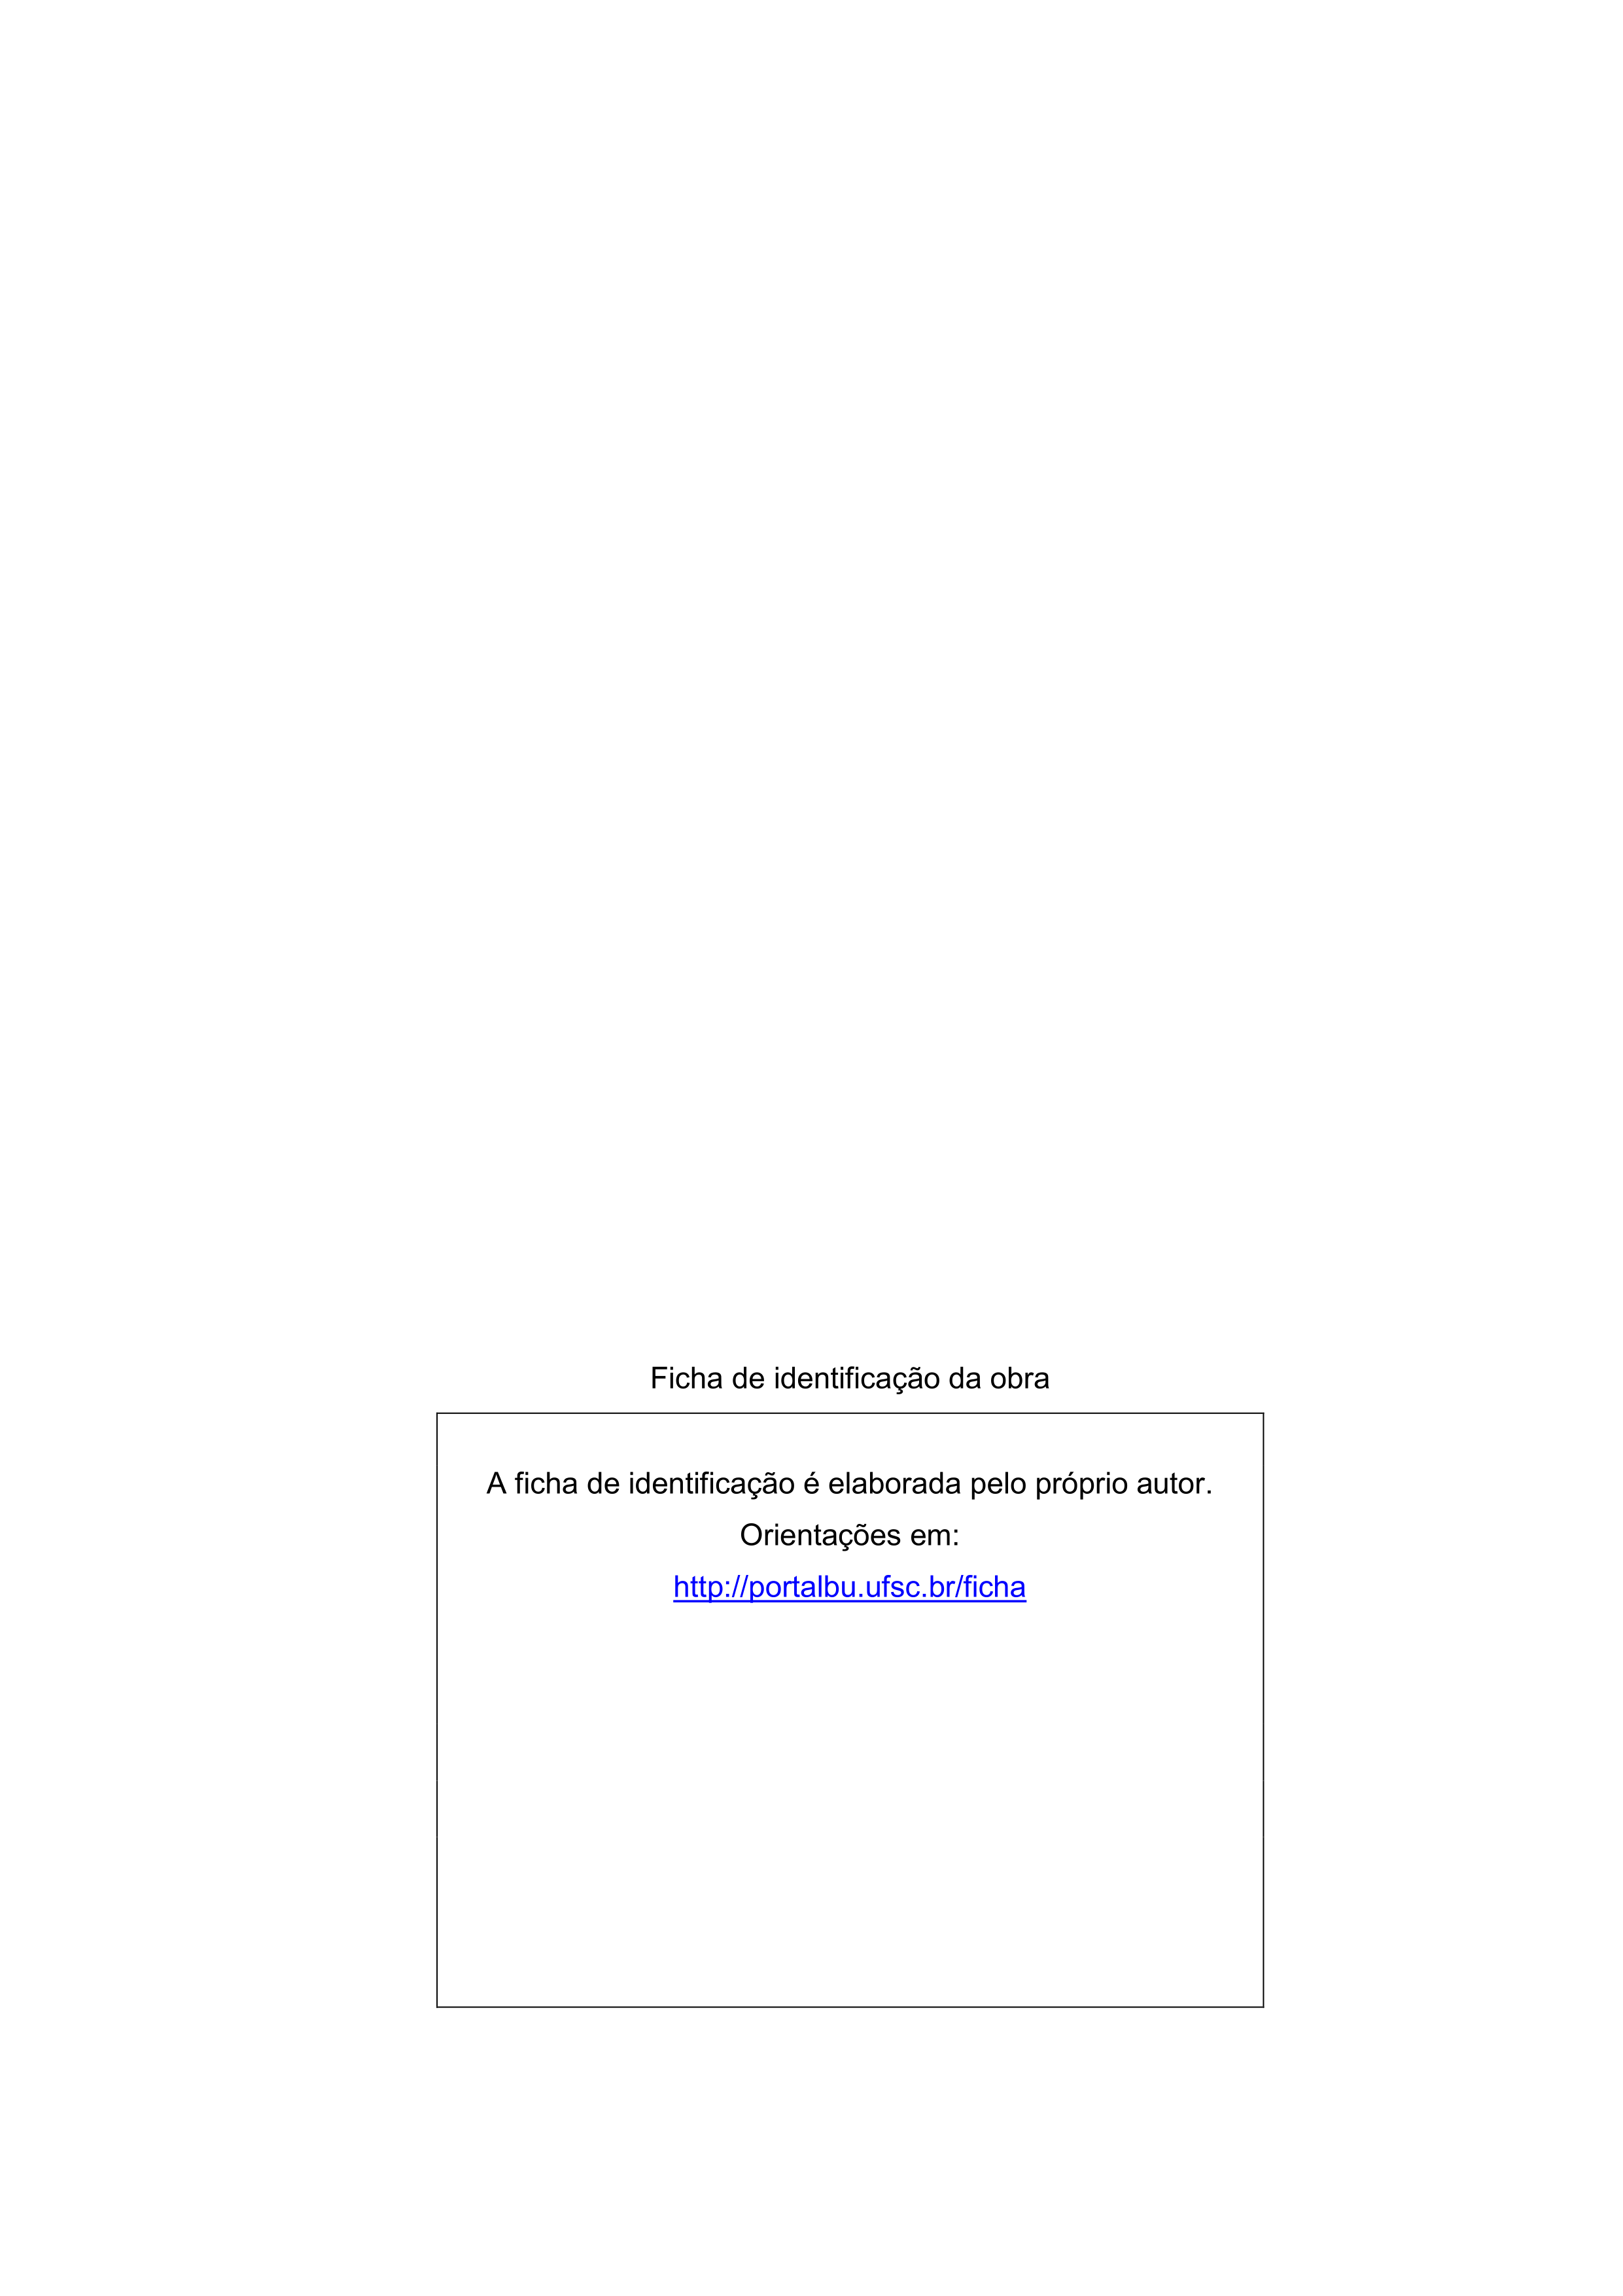
\includegraphics[width=\textwidth,height=0.85\textheight,keepaspectratio]{beforetext/Ficha_Catalografica.png}
	\end{center}
	\vspace*{\fill}
\end{fichacatalografica}

\begin{folhadeaprovacao}
	\OnehalfSpacing
	\centering
	\imprimirautor\\
	\vspace*{10pt}
	\textbf{\imprimirtitulo}
	\ifnotempty{\imprimirsubtitulo}{:~\imprimirsubtitulo}\\
	\vspace*{\baselineskip}
	O presente trabalho em nível de \imprimirnivel~foi avaliado e aprovado, em \imprimirdata, pela banca examinadora composta pelos seguintes membros:\\
	\vspace*{\baselineskip}
	Prof.(a) xxxx, Dr(a).\\
	Instituição xxxx\\
	\vspace*{\baselineskip}
	Prof.(a) xxxx, Dr(a).\\
	Instituição xxxx\\
	\vspace*{\baselineskip}
	Prof.(a) xxxx, Dr(a).\\
	Instituição xxxx\\
	\vspace*{2\baselineskip}
	\begin{minipage}{\textwidth}
		Certificamos que esta é a \textbf{versão original e final} do trabalho de conclusão que foi julgado adequado para obtenção do título de \imprimirformacao.\\
	\end{minipage}
	\vspace*{\fill}
	\assinatura{\OnehalfSpacing Coordenação do Programa de Pós-Graduação}
	\vspace*{\fill}
	\assinatura{\OnehalfSpacing\imprimirorientador \\ \imprimirorientadorRotulo}
	\vspace*{\fill}
	\imprimirlocal, \imprimirano.
\end{folhadeaprovacao}

% TODO: Dedicar
\begin{dedicatoria}
	\vspace*{\fill}
	\noindent
	\begin{adjustwidth*}{}{5.5cm}
		\raggedleft
		...
	\end{adjustwidth*}
\end{dedicatoria}

% TODO: Agradecer
\begin{agradecimentos}
    ...
\end{agradecimentos}

% TODO: Epigrafar
\begin{epigrafe}
	\vspace*{\fill}
	\begin{flushright}
		\textit{...}
	\end{flushright}
\end{epigrafe}

% TODO: Resumir
\setlength{\absparsep}{18pt}
\begin{resumo}
	\SingleSpacing
    ...
	
	\textbf{Palavras-chave}: ...
\end{resumo}

% TODO: Summarize
\begin{resumo}[Abstract]
	\SingleSpacing
	\begin{otherlanguage*}{english}
        ...

		\textbf{Keywords}: ...
	\end{otherlanguage*}
\end{resumo}

{
	\hypersetup{hidelinks}
	\pdfbookmark[0]{\listfigurename}{lof}
	\listoffigures*
	\cleardoublepage
	
	\pdfbookmark[0]{\listofquadrosname}{loq}
	\listofquadros*
	\cleardoublepage
	
	\pdfbookmark[0]{\listtablename}{lot}
	\listoftables*
	\cleardoublepage
	
	\imprimirlistadesiglas
	
	\imprimirlistadesimbolos
	
	\pdfbookmark[0]{\contentsname}{toc}
	\tableofcontents*
	\cleardoublepage
}


\textual
\setcounter{table}{0}

\chapter{Introduction}

% What are RTOS?
% TODO: Cite the definition of RTOS
Currently, several areas of technology require software that must execute in real-time. This often includes autonomous vehicles, aviation, robotics, industrial systems, and other critical systems where the software is directly responsible for system safety and control. In these domains, a failure to meet timing constraints during execution can lead to severe consequences. Thus, to ensure predictable execution and meet these timing requirements, \glspl{rtos} are utilized.

% Some common constraints and why they could be addressed with utilization prediction
% TODO: Cite thermal constraints
% TODO: Cite DVFS
% WARN: This "safer" here is doing some heavy lifting
These systems are commonly employed in embedded scenarios, where other variables must also be considered, such as energy consumption and thermal limits \cite{rahim2025survey}. \gls{dvfs} can be used to reduce the energy consumption, but, to be used in a \gls{rtos}, there must be a careful consideration for the timing constraints and how different \gls{dvfs} levels can alter the utilization of tasks. An algorithm for task utilization prediction could be employed to address this concern, enabling the safer usage of \gls{dvfs}, Since the utilization observed in the current \gls{dvfs} level does not transfer directly to other levels, it must be predicted before any level change. Moreover, task utilization prediction can be useful for other applications, such as load balancing, where an estimation of utilization could be made for different task configurations.

% Why prediction isn't easy and this is a problem
% WARN: Something here feels off, maybe the jump from prediction to the problems is just too quick?
However, predicting the utilization is a considerable challenge in modern multicore systems \cite{ul2018task, hoffmann2021online}. One of the major challenges introduced by multicore processors is interference, which arises from task contention for shared resources such as main memory, caches, and I/O peripherals. This contention introduces non-deterministic delays into task execution, making it difficult to accurately estimate the execution times and the overall utilization \cite{gracioli2019designing, horstmann2019framework, aceituno2023optimized, lugo2022survey} with the usage of simple analytical methods. The problem is aggravated in heterogeneous multicore processors, which display cores with different characteristics \cite{mrabet2024scheduling, jadon2024comprehensive}.

% TODO: Maybe add another section explaining that using PMCs is a better idea than just using system metrics

% What some people tried and why it is still not working so well
% WARN: This is undersourced
% WARN: das2019sok isn't focused on prediction, cite something else too
In recent years, several works have proposed the use of \glspl{pmc} in predictive algorithms, relying on hardware information to guide decisions. Most of these approaches rely on \gls{ml} techniques, however, they also report difficulties and pitfalls that hinder their adoption. \gls{ml} solutions usually introduce prohibitive overhead and fail to generalize well to new task-sets and platforms \cite{rahim2025survey}. Moreover, the use of \glspl{pmc} makes it difficult to design portable predictive algorithms. Although some works propose solutions to this issue, they remain limited by problems such as the divergence of \gls{pmc} semantics across architectures, lack of counters in some platform implementations and also noise introduced by the \gls{os} and other external sources \cite{das2019sok}.

% What we will do
% TODO: Detail more the solution in the future
Considering this scenario, it would be useful to address the main problems associated with the use of predictive algorithms in \gls{rtos}, specifically with the usage of \gls{pmc} enabled \gls{ml} based algorithms. This dissertation focuses on these problems and offers an analysis based on data collected from a \gls{rtos} running on multicore RISC-V and ARM platforms, with an additional proposed solution that improves upon the current approaches and offers a portable \gls{ml} guided, \gls{pmc} enabled, multicore capable, predictive algorithm applied to energy consumption optimization and load balancing. The proposed solution employs lightweight task-local \gls{ml} models executed in idle time for minimal interference with the tasks.

% TODO: In the future, add the results here

% TODO: Check the section names
\section{Objectives}

The sections below present the general and specific objectives.

\subsection{General Objective}

The objective of this work is to improve upon the current approaches to task utilization prediction by developing a portable algorithm for utilization prediction in multicore systems with the usage of \gls{ml} models and \gls{pmc}. The main focus will be in the usage of this algorithm for energy optimization and load balancing.

\subsection{Specific Objectives}

% WARN: This is quite simple, maybe there should be some refinement
\begin{itemize}
    \item Provide an evaluation of common problems in statistical approaches to utilization prediction in multicore RISC-V platforms, evaluating the performance of the approach of \textcite{hoffmann2021online};
    \item Provide an implementation of a \gls{ml} guided portable algorithm for utilization prediction in multicore systems with the use of \gls{pmc}, with the focus in energy optimization and load balancing;
    \item Perform an evaluation of the implementation in a RISC-V platform;
    \item Perform an evaluation of the implementation in an ARM platform.
\end{itemize}


\chapter{Theoretical Basis}\label{cap:theory}

...


\chapter{Conclusion}

...


\begingroup
    \SingleSpacing\printbibliography
\endgroup

\begin{apendicesenv}
	\counterwithin{figure}{chapter}
	\chapter{Appendix}

...

\end{apendicesenv}

\begin{anexosenv}
	\chapter{Annex}

...

\end{anexosenv}

\end{document}
